% !TEX root = ../Thesis.tex


\subtitle{}
\date{April 29, 2020}

%% TODO: This needs to be shortened a bit. In 2013, this lecture was
%% 5-10 minutes too long (I managed it in one session but ran over)
%% without being too slow or too fast. We can probably get rid of the
%% 15-puzzle stuff, moving it to the exercises to make some time. And
%% a not-RPG-centric description of h^max/h^add/h^FF could probably
%% also be done faster than the current RPG-centric one.

\usetikzlibrary{shapes}

\tikzstyle{relaxed planning graph}=[draw,inner sep=0pt,font=\small]
\tikzstyle{rpg square}=[relaxed planning graph,minimum size=0.52cm,rectangle]
\tikzstyle{rpg circle}=[relaxed planning graph,minimum size=0.52cm,circle]

\tikzstyle{prop}=        [rpg circle,fill=yellow]
\tikzstyle{notthere}=    [color=gray!15,fill=gray!5]
\tikzstyle{operator}=    [rpg square,fill=blue!40]
\tikzstyle{selected}=[fill=cyan]

\tikzstyle{goalachieved}=[fill=red!50]
\tikzstyle{solved} = [fill=green!30]
\tikzstyle{assignedprop}=[rpg circle,fill=orange!40]
\tikzstyle{assignedoperator}=[rpg square,fill=orange!40]

\tikzstyle{idle}=[thin]
\tikzstyle{nonidle}=[thin]
\tikzstyle{arc selected}=[color=cyan,very thick]

\newcommand{\markplusone}[1]{\path (#1) +(-0.04cm,0.28cm) node {\tiny $+1$};}
\newcommand{\markopnode}[3][0.35cm]{\path (#2) +(0cm,#1) node {\tiny
    \ensuremath{#3}};}
\newcommand{\markopnodeff}[3][0.30cm]{\path (#2) +(0cm,#1) node {\tiny
    \ensuremath{#3}};}
\newcommand{\markopcost}[2]{\path (#1) +(0.45cm,0.15cm) node {\tiny $+#2$};}

\newcommand{\pre}{\ensuremath{\textit{pre}}}
\newcommand{\add}{\ensuremath{\textit{add}}}
\newcommand{\del}{\ensuremath{\textit{del}}}
\newcommand{\relaxation}[1]{\ensuremath{#1^+}}
\newcommand{\hplus}{\ensuremath{h^+}}
\newcommand{\hmax}{\ensuremath{h^{\textup{max}}}}
\newcommand{\hadd}{\ensuremath{h^{\textup{add}}}}
\newcommand{\hff}{\ensuremath{h^{\textup{FF}}}}



  %% TODO: Got rid of centering to avoid the graph jumping.
  %% Should find a better solution for this.
  %% \begin{center}
\begin{center}
\begin{minipage}[t]{.7\linewidth}
\vspace{8pt}
\centering
\begin{frame}{}
    \begin{tikzpicture}
      \pgfsetxvec{\pgfpoint{2.77cm}{0.0cm}}
      \pgfsetyvec{\pgfpoint{0.0cm}{0.87cm}}
      %% variable layer 0
      \only<1->{
        \node[prop, solved] at (0.0,7.0) (a0) {0};
        \node[prop, solved] at (0.0,6.0) (b0) {0};
        \node[prop, notthere] at (0.0,5.0) (c0) {$c^0$};
        \node[prop,notthere] at (0.0,4.0) (d0) {$d^0$};
        \node[prop,notthere] at (0.0,3.0) (e0) {$e^0$};
        \node[prop,notthere] at (0.0,2.0) (f0) {$f^0$};
        \node[prop,notthere] at (0.0,1.0) (g0) {$g^0$};
        \node[prop,notthere] at (0.0,0.0) (h0) {$h^0$};
      }
      %% action layer 1
      \only<2->{
        %% action a_1
        \node[operator, solved] at (0.5,6.5) (o1-1) {1};
        \markopcost{o1-1}{1};
        \draw[->,nonidle] (a0)--(o1-1);
        \node[operator, solved] at (0.5,3.5) (o4-1) {1};
        \markopcost{o4-1}{1};
        \draw[->,nonidle] (b0)--(o4-1);
      }
      %% variable layer 1
      \only<3->{
        \node[prop, solved] at (1.0,7.0) (a1) {0};
        \node[prop, solved] at (1.0,6.0) (b1) {0};
        \node[prop, solved] at (1.0,5.0) (c1) {2};
        \node[prop,notthere] at (1.0,4.0) (d1) {$d^1$};
        \node[prop,notthere] at (1.0,3.0) (e1) {$e^1$};
        \node[prop, solved] at (1.0,2.0) (f1) {2};
        \node[prop,notthere] at (1.0,1.0) (g1) {$g^1$};
        \node[prop,notthere] at (1.0,0.0) (h1) {$h^1$};
        %% idle arcs
        \draw[->,idle] (a0)--(a1);
        \draw[->,idle] (b0)--(b1);
        \draw[->,idle,notthere] (c0)--(c1);
        \draw[->,idle,notthere] (d0)--(d1);
        \draw[->,idle,notthere] (e0)--(e1);
        \draw[->,idle,notthere] (f0)--(f1);
        \draw[->,idle,notthere] (g0)--(g1);
        \draw[->,idle,notthere] (h0)--(h1);
        %% effect arcs
        \draw[->,nonidle] (o1-1)--(b1);
        \draw[->,nonidle] (o1-1)--(c1);
        \draw[->,nonidle] (o4-1)--(f1);
      }
      %% action layer 2
      \only<4->{
        %% action a_1
        \node[operator, solved] at (1.5,6.5) (o1-2) {1};
        \markopcost{o1-2}{1};
        \draw[->,nonidle] (a1)--(o1-2);
        %% action a_2
        \node[operator, solved] at (1.5,5.5) (o2-2) {3};
        \markopcost{o2-2}{1};
        \draw[->,nonidle] (a1)--(o2-2);
        \draw[->,nonidle] (c1)--(o2-2);
        %% action a_3
        \node[operator, solved] at (1.5,4.5) (o3-2) {3};
        \markopcost{o3-2}{1};
        \draw[->,nonidle] (b1)--(o3-2);
        \draw[->,nonidle] (c1)--(o3-2);
        %% action a_4
        \node[operator, solved] at (1.5,3.5) (o4-2) {1};
        \markopcost{o4-2}{1};
        \draw[->,nonidle] (b1)--(o4-2);
      }
      %% variable layer 2
      \only<5->{
        \node[prop, solved] at (2.0,7.0) (a2) {0};
        \node[prop, solved] at (2.0,6.0) (b2) {0};
        \node[prop, solved] at (2.0,5.0) (c2) {2};
        \node[prop, solved] at (2.0,4.0) (d2) {4};
        \node[prop, solved] at (2.0,3.0) (e2) {4};
        \node[prop, solved] at (2.0,2.0) (f2) {2};
        \node[prop,notthere] at (2.0,1.0) (g2) {$g^2$};
        \node[prop,notthere] at (2.0,0.0) (h2) {$h^2$};
        %% effect arcs
        \draw[->,nonidle] (o1-2)--(b2);
        \draw[->,nonidle] (o1-2)--(c2);
        \draw[->,nonidle] (o2-2)--(d2);
        \draw[->,nonidle] (o3-2)--(e2);
        \draw[->,nonidle] (o4-2)--(f2);
        %% idle arcs
        \draw[->,idle] (a1)--(a2);
        \draw[->,idle] (b1)--(b2);
        \draw[->,idle] (c1)--(c2);
        \draw[->,idle,notthere] (d1)--(d2);
        \draw[->,idle,notthere] (e1)--(e2);
        \draw[->,idle] (f1)--(f2);
        \draw[->,idle,notthere] (g1)--(g2);
        \draw[->,idle,notthere] (h1)--(h2);
      }
      %% action layer 3
      \only<6->{
        %% action a_1
        \node[operator, solved] at (2.5,6.5) (o1-3) {1};
        \markopcost{o1-3}{1};
        \draw[->,nonidle] (a2)--(o1-3);
        %% action a_2
        \node[operator, solved] at (2.5,5.5) (o2-3) {3};
        \markopcost{o2-3}{1};
        \draw[->,nonidle] (a2)--(o2-3);
        \draw[->,nonidle] (c2)--(o2-3);
        %% action a_3
        \node[operator, solved] at (2.5,4.5) (o3-3) {3};
        \markopcost{o3-3}{1};
        \draw[->,nonidle] (b2)--(o3-3);
        \draw[->,nonidle] (c2)--(o3-3);
        %% action a_4
        \node[operator, solved] at (2.5,3.5) (o4-3) {1};
        \markopcost{o4-3}{1};
        \draw[->,nonidle] (b2)--(o4-3);
        %% action a_5
        \node[operator, solved] at (2.5,2.5) (o5-3) {5};
        \markopcost{o5-3}{1};
        \draw[->,nonidle] (d2)--(o5-3);
        %% action a_6
        \node[operator, solved] at (2.5,1.5) (o6-3) {5};
        \markopcost{o6-3}{1};
        \draw[->,nonidle] (d2)--(o6-3);
      }
      %% variable layer 3
      \only<7->{
        \node[prop, solved] at (3.0,7.0) (a3) {0};
        \node[prop, solved] at (3.0,6.0) (b3) {0};
        \node[prop, solved] at (3.0,5.0) (c3) {2};
        \node[prop, solved] at (3.0,4.0) (d3) {4};
        \node[prop, solved] at (3.0,3.0) (e3) {4};
        \node[prop, solved] at (3.0,2.0) (f3) {2};
        \node[prop, solved] at (3.0,1.0) (g3) {6};
        \node[prop,notthere] at (3.0,0.0) (h3) {$h^3$};
        %% effect arcs
        \draw[->,nonidle] (o1-3)--(b3);
        \draw[->,nonidle] (o1-3)--(c3);
        \draw[->,nonidle] (o2-3)--(d3);
        \draw[->,nonidle] (o3-3)--(e3);
        \draw[->,nonidle] (o4-3)--(f3);
        \draw[->,nonidle] (o5-3)--(e3);
        \draw[->,nonidle] (o5-3)--(f3);
        \draw[->,nonidle] (o6-3)--(g3);
        %% idle arcs
        \draw[->,idle] (a2)--(a3);
        \draw[->,idle] (b2)--(b3);
        \draw[->,idle] (c2)--(c3);
        \draw[->,idle] (d2)--(d3);
        \draw[->,idle] (e2)--(e3);
        \draw[->,idle] (f2)--(f3);
        \draw[->,idle,notthere] (g2)--(g3);
        \draw[->,idle,notthere] (h2)--(h3);
      }
      \only<beamer:8|handout:0>{
        \node[prop,solved] at (3.0,5.0) (c3) {2};
        \node[prop,solved] at (3.0,4.0) (d3) {4};
        \node[prop,solved] at (3.0,3.0) (e3) {4};
        \node[prop,solved] at (3.0,2.0) (f3) {2};
        \node[prop,solved] at (3.0,1.0) (g3) {6};
      }
      \only<9->{
        \node[operator,goalachieved] at (3.5,3.0) (G) {18};
        \draw[->,nonidle] (c3)--(G);
        \draw[->,nonidle] (d3)--(G);
        \draw[->,nonidle] (e3)--(G);
        \draw[->,nonidle] (f3)--(G);
        \draw[->,nonidle] (g3)--(G);
      }
    \end{tikzpicture}
  % $\hadd(s') = 34/2 = 9$
  %% \end{center}
   %% \end{center}
\end{frame}
\end{minipage}%
\begin{minipage}[t]{.4\linewidth}
\vspace{-30pt}
\centering
\begin{longtable}[c]{| c | c | c|}
     \hline
     \multicolumn{3}{| c |}{new state $s$}\\
     \hline
     $q$ & $x_q$ & $rhs_q$\\
     \hline
     \endfirsthead
     \hline
     \endfoot
     $a$ & 0 & 0\\
     $b$ & 0 &  \textcolor{red}{2}\\
     $c$ & 2 & \textcolor{red}{0}\\
     $d$ & 4 & 4\\
     $e$ & 4 & 4\\
     $f$ & 2 & 2\\
     $g$ & 6 & 6\\
     $a_1$ & 1 & 1\\
     $a_2$ & 3 & 3\\
     $a_3$ & 3 & 3\\
     $a_4$ & 1 & 1\\
     $a_5$ & 5 & 5\\
     $a_6$ & 5 & 5\\
     \hline
\end{longtable}
\end{minipage}
\end{center}

